\subsection{Reporting}

The second goal of this project is to provide parents with the ability to
monitor and derive reports on their child's Internet access. 
%
We looked at incorporating BASE (Basic Analysis and Security Engine) into Kindsicher to
render this functionality. 
%
BASE is based of the ACID (Analysis Console for Intrusion Databases) project
and provides a web-based front-end to query and analyze alerts generated by
the SNORT IDS system.

We first define a rule within SNORT to capture all HTTP traffic originating
from the home network.  

\verb+alert tcp any any <> any 80 (msg:"HTTP Alert")+ 

This causes SNORT to log all HTTP requests from any source IP and port to any
destination IP and port 80 (indicating HTTP) to a MySQL database. 
%
BASE then reads the alert information from this database and displays it in a
web-browser. (Figure R1)

\begin{figure}
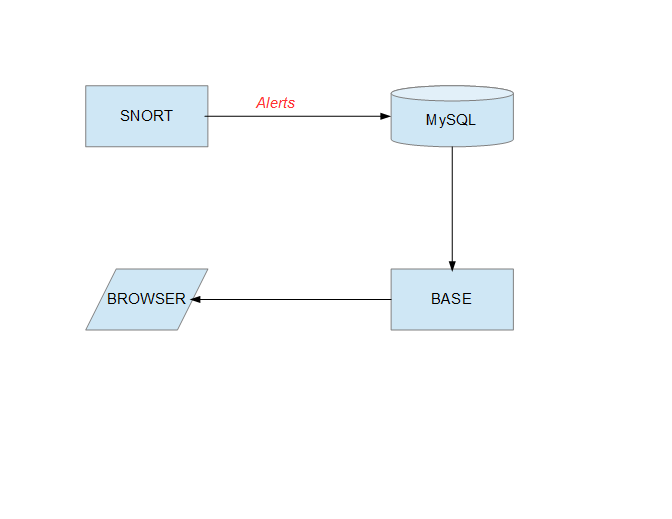
\includegraphics{figures/R1_BASE_Flow}
\end{figure}

% TODO: do something to label this R1 or similar

To access base you need to open a browser window and type in “<base server
name>/base” in the URL field.
%
Figure R2 shows the BASE home page presented to an user on logging into BASE.
